\documentclass[11pt,a4j,fleqn]{jarticle}
\usepackage{amsmath,amsthm,amssymb}
\usepackage[dvipdfmx]{graphicx}
\usepackage{ascmac}

\title{包絡線定理}
\author{辻 裕一郎}
\date{2014/6/7}


\begin{document}

\maketitle

\section{はじめに}
今回は、『経済セミナー』に掲載されている包絡線の図をPythonで描け、という課題であった。
そもそも包絡線定理について完全に理解している訳でもないのに、
どうすればいいのか分からないこともあって相当苦労した覚えしかない。

多大な手助けをいただいた尾山先生、ゼミ生のみなさんには大いに感謝したい。

\section{包絡線定理}

次のような関数を考える。
\begin{equation}
f(x, t) =  tx -t^2 
\end{equation}

まず、これを $x$ の関数とみると、これは傾きが $t$ 、切片が $-t^2$ の直線になる。
例えば $t = 1$ とすると、 $f(x, 1) = x - 1 $ という直線になる。
$t$ の値をいろいろ変えて直線を何本も引いてみると、次のページの図1、図2のようになる。

これを見ると、直線の通過領域は「ある曲線」の下側全体になっていることがわかる。
よって、この「ある曲線」を表す関数を $ F (x) $ とおくと、
\begin{equation}
F(x) = \max_{t} {f(x , t)}
\end{equation}
となる。
$f(x, t)$ において $x$ を変数、$t$ をパラメータとみて平方完成を行うと
\begin{equation}
 f(x, t) = -\left(t - \frac{x}{2}\right)^2 + \frac{x^2}{4} 
\end{equation}
となるから、$f$ は $ t = x / 2 $ で最大値 $ x^2 / 4 $を取ることが分かる。
従って、 $F(x) = x^2/4$ である。 この時、曲線 $F(x)$ は直線群の包絡線(envelope)であるという。

\newpage

\begin{figure}[htbp]
  \begin{center}
    \begin{tabular}{c}

      % 1
      \begin{minipage}{0.33\hsize}
        \begin{center}
          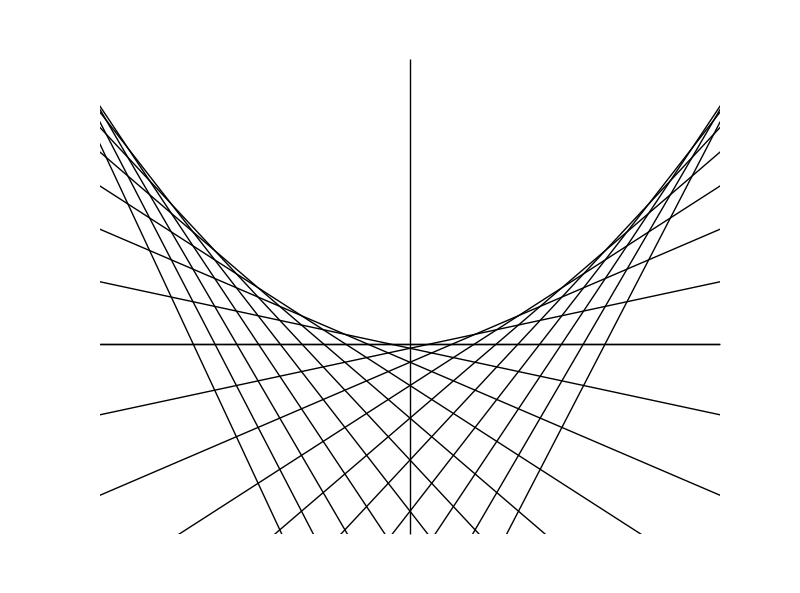
\includegraphics[bb=0 0 240 180 , width=3cm]{envelope1.png}
          \hspace{1.6cm} [1]包絡線(1)
        \end{center}
      \end{minipage}

      % 2
      \begin{minipage}{0.33\hsize}
        \begin{center}
          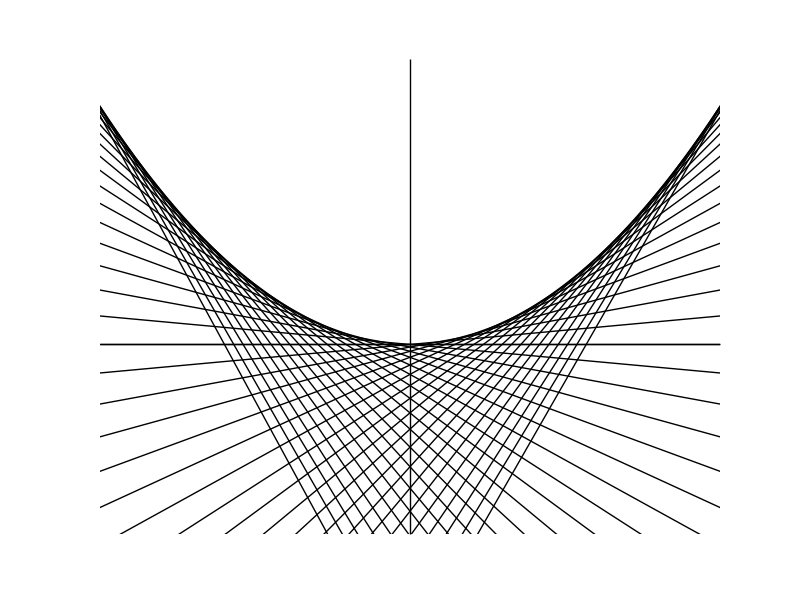
\includegraphics[bb=0 0 240 180 , width=3cm]{envelope0.png}
          \hspace{1.6cm} [2]包絡線(2)
        \end{center}
      \end{minipage}

    \end{tabular}
    \caption{包絡線定理}
    \label{envelope}
  \end{center}
\end{figure}

また、各直線は包絡線と接しているということも確かめられる。
実際、最大化問題の解を$x$に依存する形で $t^*(x)$ と書くと、
各 $x = \bar{x}$ において $F(\bar{x}) = f(\bar{x} , t^*(\bar{x}))$ であるから、
直線と包絡線は $x = \bar{x}$で交わる。
また、曲線の $x = \bar{x}$ における傾きは $F^{'}(\bar{x}) = x/2$、
直線の傾きは$t = x/2$であるから、両者の傾きは等しい。
故に、両曲線は $x = \bar{x}$で接する。

\vspace{0.3cm}

ここから、最大化問題の価値関数 $F(x)$ を微分するには、最適解を代入してからパラメータで微分しても、
パラメータで微分してから最適解を代入しても結果は同じになる、ということがわかる。

\vspace{0.3cm}

これは、この場合に限らず一般的に成り立つ命題であり、包絡線定理(envelope theorem)と呼ばれる。
厳密な定義は以下のようになる。

\vspace{0.3cm}

\begin{itembox}[1]{ \Large 【定理1.】  包絡線定理}
 関数$f(x , t) $について、$t$を変数、$x$をパラメータとし,その最大化問題の解関数を$t^*(x)$、
 価値関数$F(x)$とする。すなわち、
 \[F(x) = \max_{t} {f(x,t)} = f(x , t^*(x))\]
 である。
 さらに、$F(x)$と$f(x,t)$は$x$について微分可能とする。このとき、次が成り立つ。
 \begin{equation}
  F^{'}(x) = \frac{\partial f}{\partial t} (x , t^*(x))
 \end{equation}
\end{itembox}

\vspace{0.3cm}

\newpage

\section{Pythonプログラム}

このような性質を持つ包絡線を描くため、Pythonで以下のようなプログラムを組んだ。

\begin{quote}
\begin{verbatim}
# -*- coding: utf-8 -*-
import matplotlib.pyplot as plt
import numpy as np
def f(x,t):
    return t*x-t**2 #関数を設定
def subplots():
    fig, ax = plt.subplots()
    for spine in ['left', 'bottom']:
        ax.spines[spine].set_position('zero') #左と下の軸は中央に
    for spine in ['right', 'top']:
        ax.spines[spine].set_color('none') #右と上の軸は色を消す
    ax.set_xticks([]) #x軸の目盛りを消す
    ax.set_yticks([]) #y軸の目盛りを消す
    return (fig, ax)

fig, ax = subplots()
x = np.linspace(-10, 10, 200) #xの範囲を決める

FILEFORMAT = 'png'  # 'png' or 'pdf'
FIGNUM = 0  # 0 (細かい) or 1 (粗い)

if FIGNUM == 0:  # envelope0(細かい)
    for s in range(-20, 20 + 1): #tでループさせる値を決める
        t = s * 0.3
        y = f(x, t)
        ax.plot(x, y, 'k-', linewidth=1)

if FIGNUM == 1:  # envelope1(粗い)
    for s in range(-10, 10 + 1): #tでループさせる値を決める
        t = s * 0.5
        y = f(x, t)
        ax.plot(x, y, 'k-', linewidth=1)

plt.ylim(-20, 30) #yの表示範囲を決める
plt.savefig('envelope' + str(FIGNUM) + '.' + FILEFORMAT)  #出力する
plt.show()
\end{verbatim}
\end{quote}

\section{おわりに}
包絡線の図をPythonでプログラムを組んでみたが、自分でゼロからできることは非常に少なく、
尾山先生や他のゼミ生に助けてもらいながらの作成となった。
今後はもう少し自分の力で書けるようにしていきたいと思う。

今後の改善点としては、関数のパラメータの値をforループで回すコードをもっとスマートにすること、
また軸に矢印を付けたりして座標をもっと分かりやすく書くこと、といった点である。
Python全体に関する勉強だけでなく、個別の関数に関する知識も増やしていくようにしたい。

\begin{thebibliography}{0}
\bibitem{OyamaYasuda11}
尾山大輔・安田洋祐「経済学で出る包絡線定理」『経済セミナー』2011年10・11月号.
\bibitem{ItoKose}
伊藤幹夫・戸瀬信之『経済学とファイナンスのための基礎数学』
\bibitem{lecturenote}
2014夏学期「経済学のための数学」講義ノート
\end{thebibliography}

\end{document}